\documentclass[a4paper,12pt]{article}
\usepackage{times}  % DO NOT CHANGE THIS
\usepackage{helvet} % DO NOT CHANGE THIS
\usepackage{courier}  % DO NOT CHANGE THIS
\usepackage[hyphens]{url}  % DO NOT CHANGE THIS
\usepackage{graphicx} % DO NOT CHANGE THIS
\urlstyle{rm} % DO NOT CHANGE THIS
\def\UrlFont{\rm}  % DO NOT CHANGE THIS
\usepackage{natbib}  % DO NOT CHANGE THIS AND DO NOT ADD ANY OPTIONS TO IT
\usepackage{caption} % DO NOT CHANGE THIS AND DO NOT ADD ANY OPTIONS TO IT
\frenchspacing  % DO NOT CHANGE THIS
\setlength{\pdfpagewidth}{8.5in}  % DO NOT CHANGE THIS
\setlength{\pdfpageheight}{11in}  % DO NOT CHANGE THIS
\usepackage{algorithm} %format of the algorithm 
\usepackage{algorithmic} %format of the algorithm 
\usepackage{multirow} %multirow for format of table 
\usepackage{amsmath} 
\usepackage{xcolor}
\usepackage{amssymb}
\usepackage{enumerate}
\usepackage{amsmath}
\usepackage{xeCJK}
\usepackage{courier}
\DeclareMathOperator*{\argmax}{argmax} % thin space, limits underneath in displays

\begin{document}

\title{强化学习:作业四}

\author{杨思航 191180166}

\date{\today}

\maketitle

\section{作业内容}
在 gridworld 环境下实现 Model-based Q-learing 算法。

\section{实验环境}
\begin{itemize}
    \item NAME = Ubuntu
    \item VERSION = 20.04.2 LTS(Focal Fossa)
    \item Tensorflow = 2.7.0
\end{itemize}

\section{实验探究}
\begin{enumerate}
    \item Dyna-Q 算法
    \begin{enumerate}[(1)]
        \item 核心代码
        \begin{itemize}
            \item policy 的学习部分基于 HW2, 但是将 observation 从三维映射到一维以便于后续 model 的学习
            \item DynaModel 的实现借鉴了框架代码中的 NetworkModel
            \item 具体实现流程请见 algo.py -> DynaModel
        \end{itemize}
        \newpage
        \item 参数 $n$ 对算法收敛性的影响
        \begin{itemize}
            \item 收敛 
            \begin{enumerate}
                \item 由于框架代码并未显示定义收敛, 因此我自行定义了收敛
                \item $\text{converge\_threshold}=87$, $87$ 为最优解于最坏初始情况\\
                (距离钥匙和门的距离之和最大)下的奖赏
                \item 若连续 $10$ 次测试均满足 $\min(\text{reward\_episode\_set})\geq$\\
                $\text{converge\_threshold}$, 则认为算法收敛
            \end{enumerate}
            \item 实验结果
            \begin{enumerate}
                \item 收敛时间 \\
                (曲线呈现增长趋势的原因: 学习模型需要额外消耗时间)
                \begin{figure*}[h!]
                    \centering
                    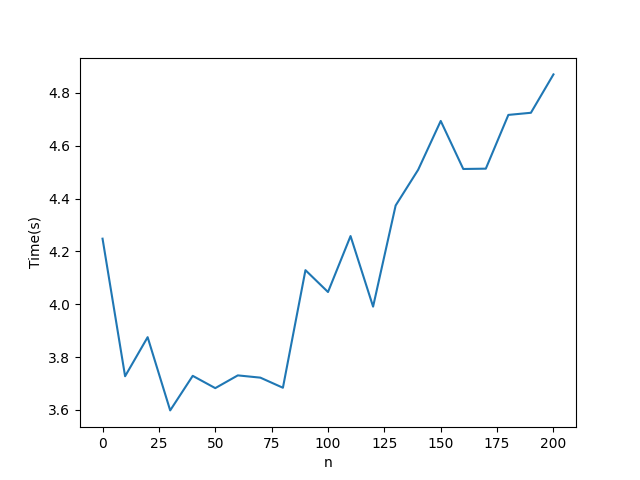
\includegraphics[scale=0.45]{pics/1-time.png}
                \end{figure*}
                \item 消耗的样本量 (Total Steps) \\
                (对于每一个 $n$ 重复执行 $10$ 次取平均值, 由于学习存在随机性, 因此曲线存在小幅度震荡)
                \begin{figure*}[h!]
                    \centering
                    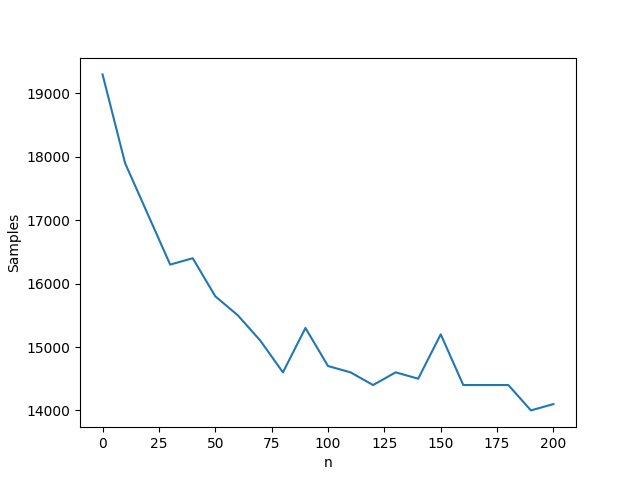
\includegraphics[scale=0.45]{pics/1-sample.png}
                \end{figure*}
            \end{enumerate}
            \item 实验结论: 当 $n=120$ 时, 收敛时所消耗的样本数量基本趋于稳定, 不再呈明显下降趋势
        \end{itemize}
    \end{enumerate}
    \item NetworkModel
    \begin{enumerate}[(1)]
        \item 
    \end{enumerate}
\end{enumerate}

\section{实验效果}
\section{复现实验}
\section{小结}

\end{document}